\documentclass[11pt]{article}
\usepackage[margin=0.9in]{geometry}
\usepackage{amsmath,booktabs,graphicx,hyperref}
\hypersetup{hidelinks}
\title{Can a screening threshold travel between hospitals?\\A compact CNN study on chest radiographs}
\author{Mathematics Behind AI project team}
\date{}
\begin{document}
\maketitle
\begin{abstract}
We trained a convolutional neural network on 496 Shenzhen radiographs and selected its screening threshold on another 166. Applied to Montgomery County, the network flagged 134 of 138 images. These included 57 of 58 TB-labeled images and 77 of 80 normal images. Removing dropout changed the net number of correct decisions by one. The high sensitivity at the second site thus came at the expense of a high false-alarm rate. We report the counts, intervals and matched differences for both models.
\end{abstract}

\section{Question}
Surulivelu et al.\ used a binarized simplicial convolutional neural network to classify radiographs after lung segmentation and feature extraction \cite{base}. We ask a narrower question about image-level classification. If a threshold is chosen at one hospital to detect at least nine in ten TB-labeled cases, how many positive cases are detected and how many normal cases are flagged at a second hospital? We compare two CNN variants and two previously measured logistic regression baselines. A direct accuracy ranking against the base paper would require its classifier to be evaluated on the same cases.

\section{Data and experimental setup}
The Shenzhen and Montgomery County collections were acquired at different sites \cite{jaeger}. We used the Kaggle distribution \cite{kaggle} and the case manifest from our earlier HOG experiment. Each source image was checked against the SHA-256 recorded in that manifest. We used the dataset's normal and TB-consistent abnormal labels. The hospital prefix and case number identify records; patient identities beyond these public identifiers cannot be audited.
\begin{center}
\begin{tabular}{lrrr}
\toprule Cohort & Normal & TB label & Total\\\midrule
Shenzhen training & 244 & 252 & 496\\
Shenzhen validation & 82 & 84 & 166\\
Montgomery external test & 80 & 58 & 138\\\bottomrule
\end{tabular}
\end{center}
We converted each radiograph to grayscale, resized it to fit a $64\times64$ canvas, scaled it between its first and 99th intensity percentiles, and zero-padded it. Downsampling makes training feasible on a CPU but can remove small findings. The classification task requires an image-level score and uses no lesion masks.

\section{Model and threshold}
The first layer learns eight $4\times4$ filters with stride four. The second learns twelve $3\times3$ filters with stride one. Both layers use ReLU. A $2\times2$ average pool reduces the activation map to $7\times7\times12$. A linear head combines these 588 features into one logit $z$. The network has 1,601 trainable parameters. For a binary label $y$, the score and the training loss are
\[
s=\frac{1}{1+e^{-z}}, \qquad \ell(z,y)=\log(1+e^z)-yz.
\]
We used Adam with a learning rate of 0.001 and a batch size of 32 for 20 epochs. Epoch 20 gave the lowest validation loss for both variants and supplied both checkpoints. No augmentation was applied. Validation guided checkpoint selection and threshold selection, so its performance describes development data.

For each model, we maximized validation specificity subject to sensitivity of at least 0.90. Ties favored higher sensitivity, then the higher threshold. A score at or above the cutoff gave a positive prediction. Both variants and their cutoffs were fixed before either CNN was scored on Montgomery. The external results from the earlier HOG experiment were already known, so this comparison remains exploratory.

\section{Ablation study}
We removed dropout from the classification head. The full network drops 35\% of pooled features during training; both variants use all features at inference. We kept the preprocessing, initialization, minibatch order, optimizer, epoch budget and checkpoint rule the same. Separate random generators for dropout masks and minibatch order allowed us to keep the batches matched. Each variant chose its own threshold under the same screening rule. We also report a common 0.5 cutoff to show how the result depends on the operating point.

\section{Cross-dataset validation}
In Shenzhen the full CNN detected 76 of 84 TB-labeled cases and correctly cleared 34 of 82 normal cases at a threshold of 0.26652. Without dropout, the corresponding counts were 77 and 39 at a threshold of 0.21648. Table~\ref{tab:external} gives the results at the second hospital. The HOG rows use the saved logistic regression runs on exactly the same cases. PCA reduced the original 1,764 HOG features to 249 components. The HOG comparisons involve changes to the whole pipeline, including the image representation.
\begin{table}[ht]\centering\small
\begin{tabular}{lrrrrrr}
\toprule Model & TP & FN & TN & FP & Sens. (\%) & Spec. (\%)\\\midrule
HOG + logistic regression &39&19&33&47&67.2&41.25\\
HOG + PCA + logistic regression &34&24&42&38&58.6&52.50\\
CNN with dropout &57&1&3&77&98.3&3.75\\
CNN without dropout &57&1&2&78&98.3&2.50\\\bottomrule
\end{tabular}
\caption{Montgomery at the Shenzhen-selected thresholds. Every row uses 58 TB-labeled and 80 normal cases.}\label{tab:external}
\end{table}

The full CNN flagged 97.1\% of the Montgomery images. A rule that flagged every image would detect all 58 TB-labeled cases and raise 80 false alarms. Relative to that rule, the full CNN cleared three normal images and missed one positive. At the common cutoff of 0.5, the full CNN detected 51 cases and raised 68 false alarms. The ablated CNN detected 51 and raised 60. External ROC AUC was 0.603 with dropout and 0.654 without, compared with 0.821 and 0.834 on Shenzhen validation. Ranking performance declined across sites even though sensitivity at the selected thresholds increased.
\begin{figure}[ht]\centering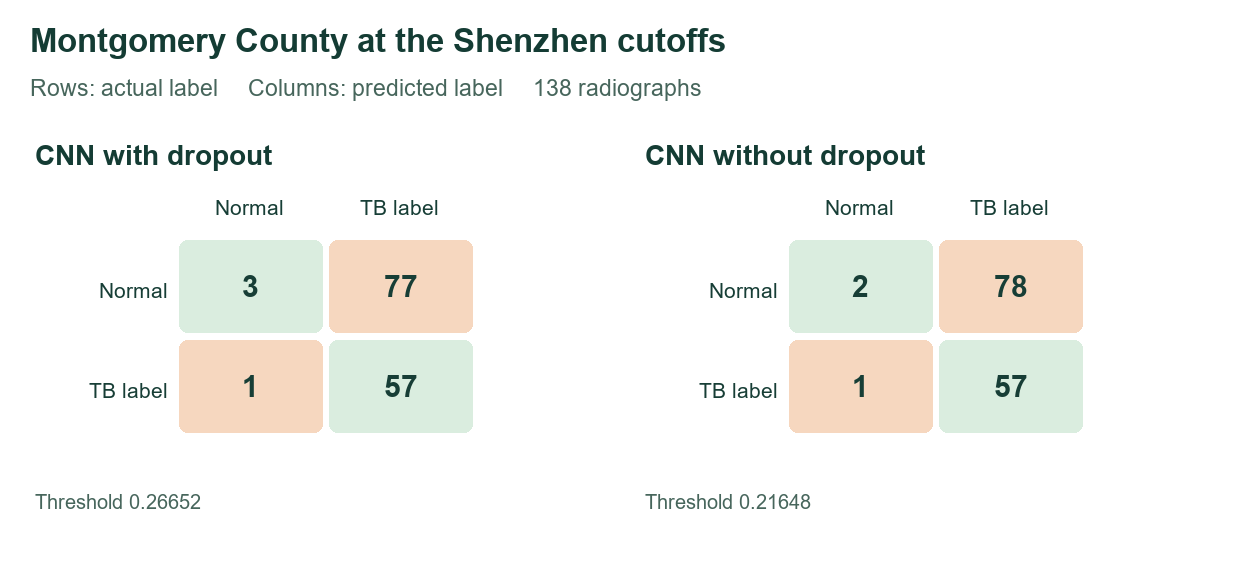
\includegraphics[width=.96\linewidth]{confusion.png}
\caption{External predictions at the cutoffs selected in Shenzhen. Rows represent actual labels.}\end{figure}

\section{Statistical analysis}
For the full CNN on Montgomery, the 95\% Wilson intervals were 90.9--99.7\% for sensitivity and 1.3--10.5\% for specificity. For the ablation, we resampled cases within each true class 5,000 times, keeping both CNN predictions for each case together. The full-minus-ablated specificity difference was 1.25 percentage points (95\% percentile interval $-2.5$ to $5.0$). The two variants made identical decisions on all 58 positives. Every paired resample of those positives therefore gave zero sensitivity difference. This describes the observed sample; population equivalence remains untested.

We used a two-sided exact McNemar test on paired correct/incorrect decisions across all 138 cases. Two disagreements favored the full CNN and one favored the ablated CNN ($p=1.00$). There is little evidence here to distinguish their overall error rates. The intervals condition on one training seed, the fitted models and the selected thresholds. They omit retraining variability.

\section{Limitations and conclusion}
Scanner settings, population composition and acquisition practices could contribute to the difference between sites. Two cohorts cannot isolate these effects. The normal comparison group also limits conclusions about discrimination from other lung diseases. A follow-up could repeat the ablation over several seeds and confirm the operating point on a previously unseen cohort. For this run, the rise in false alarms was far larger than the observed difference between the two dropout settings.

\section*{Reproduction}
The submission contains the case manifest, preprocessing and training code, both checkpoints, image-level predictions, and statistical outputs. The demo scores public dataset images with the full model at its saved cutoff. Team repository: \url{https://github.com/maahirvashisht/Tuberculosis-detection-CNN}.

\begin{thebibliography}{9}
\bibitem{base} M. Surulivelu, D. Hemanand, R. Ganesh Babu, and T.D. Subash. AI-based tuberculosis detection and localization in chest X-rays using a Binarized Simplicial Convolutional Neural Network for efficient and accurate diagnosis. \textit{Biomedical Signal Processing and Control} 113, 108928 (2026). \url{https://doi.org/10.1016/j.bspc.2025.108928}.
\bibitem{jaeger} S. Jaeger et al. Two public chest X-ray datasets for computer-aided screening of pulmonary diseases. \textit{Quantitative Imaging in Medicine and Surgery} 4, 475--477 (2014). \url{https://doi.org/10.3978/j.issn.2223-4292.2014.11.20}.
\bibitem{kaggle} N. Pandey. Chest Xray Masks and Labels, version 1. Kaggle. \url{https://www.kaggle.com/datasets/nikhilpandey360/chest-xray-masks-and-labels}.
\end{thebibliography}
\end{document}
